\section*{Quickstart}

The ViVAE is stored in free git repository at \url{http://github.com/HKou/vivae/}. The easiest way of getting it is to make git clone of the sources (assuming that you have a git tool installed in your system):

\begin{colorverbatim}
git clone git://github.com/HKou/vivae.git 
\end{colorverbatim}

Then, change to vivae directory and type:

\begin{colorverbatim}
ant
\end{colorverbatim}

to compile the sources.
An example of usage is included. It can be executed using:

\begin{colorverbatim}
ant run
\end{colorverbatim}

Normally, a java window appears (see Figure \ref{fig:intro}) and a simulation is loaded. The agents in the simulation are equipped with randomly generated fully connected recurrent neural networks that controll wheel movement based on sensory information. There are two types of sensors included in this simulation. The first type is the distance sensor. the second one is the surface sensor. Five instances of each sensor arecircularly distributed around the agents. 1000 iterations is performed and the program ends typing out the final fitness, which is the average speed of all agents in the simulation. The program outputs the following (fitness values may be different):


\begin{colorverbatim}
ant run
Buildfile: build.xml

run:
     [java] average speed fitness = 0.08090585578183623
     [java] average ontop fitness = 0.031265608469645184
\end{colorverbatim}

\begin{figure}[h!]
\centering
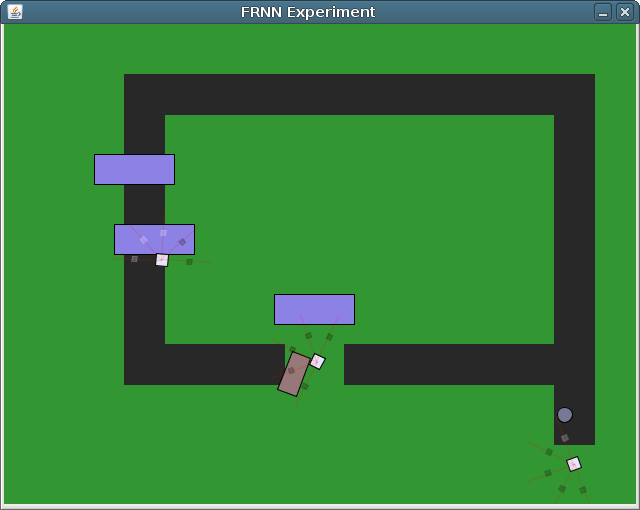
\includegraphics[width=.5\textwidth]{figures/intro}
\caption{First vivae execution. FRNNExperiment class is started, Java window appears and simulation with three agents in the arena begins. Each agent is equipped with 5 distance sensors (red lines) and 5 surface sensors (black/white) boxes. There is also two obstacles in the simulation.}
\label{fig:intro}
\end{figure}

The experiment consists of FRNN* classes in vivae.example package. FRNNExperiment class contains the main() method. FRNNController contains the recurrent neural network and controlls the agent movement. FRNNControlledRobot class is the controlled robot itself containing the sensors. The program outputs two fitness values. One is the average speed of the robots, the second one reflects how much have the obstacles been moved closer to tue upper edge of the arena.

